\chapter{Background} \label{chap:background} % 10 pages

In this chapter, we provide the background knowledge for understanding the use case and how closed-circuit television systems function and and how video data is collected, processed, and analyzed. Then in Section \ref{sec:anomaly_detection}, we provide an overview of anomaly detection and the detection techniques in that field. This also includes the highlighting of the different types of anomalies and how these appear in video streams. Lastly in Section \ref{sec:gans}, a general introduction to generative adversarial networks and the subtypes of thereof on which we build on in Chapter \ref{chap:contribution} is given.



% Closed-Circuit Television
\section{Closed-Circuit Television Systems} \label{sec:cctv}

The difference between broadcast television and closed-circuit television (CCTV), also called video surveillance, is that the video data which is transmitted is usually not broadcast, but only sent to one or multiple endpoints \cite{damjanovski2005cctv}. This definition can further be focused on camera systems that focus on the monitoring of specific places, for security or other supervision reasons. Before the spread of IP cameras, the early versions of cameras used in CCTV systems were connected to a set of monitors in centralized fashion, so human operators could monitor the different video feeds produced by the different capture sources \cite{dempsey2010introduction}. Recording and storage was done through digital video recorders (DVR)\nomenclature{DVR}{Digital video recorders}, which were later connected to the network to allow access to the video feeds from other devices. Video data was either directly processed on the DVR or the video streams were forwarded to other devices on which one could apply for example motion detection or facial recognition techniques to generate events that were of interest to the one monitoring \cite{kruegle2011cctv, bruce2001matching}.

However DVRs proofed to be single points of failure and decentralized IP cameras are these days more prevalent in their applications \cite{vlahos2009surveillance, ferenbok2013hidden}: The main advantage of this is the isolation of the different cameras from each other and that certain processing steps of the video data can be done directly on the edge where the data is being generated. In that case, the analog video signal is directly transformed to a digital one and the video camera is a device within the network that can be accessed like any other device. How the video feeds of the individual cameras can be processed differs from the CCTV system that is used \cite{fleck2010privacy}. For example, smart home surveillance cameras by Netatmo\footnote{\url{www.netatmo.com}} have a comparably small local flash memory which serves as a ring buffer, while also sending the video data to the camera provider's cloud from which the video feed can be accessed through a web interface. The data is also filtered by an event detection and facial recognition algorithm. Events (and alerts) that are generated in that manner can be forwarded to a mobile end device. In addition, the video data of any detected events can also be forwarded via FTP to another file server. 

Other products such as the ones from upCam\footnote{\url{www.upcam.de}} are more decentralized, for these cameras' video feeds and video data can be directly accessed through the cameras' web interface. Event-based filtering can also directly be done on the edge and not in the provider's cloud, that serves as a storage option. This way only actually video data that may be of interest is sent and stored. In addition, these cameras like many other IP-based ones allow the direct streaming of their video feeds to a privately managed network attached storage or other server via RTSP, as shown in Figure \ref{fig:cctv_system}.\\

\begin{figure}
	\centering
	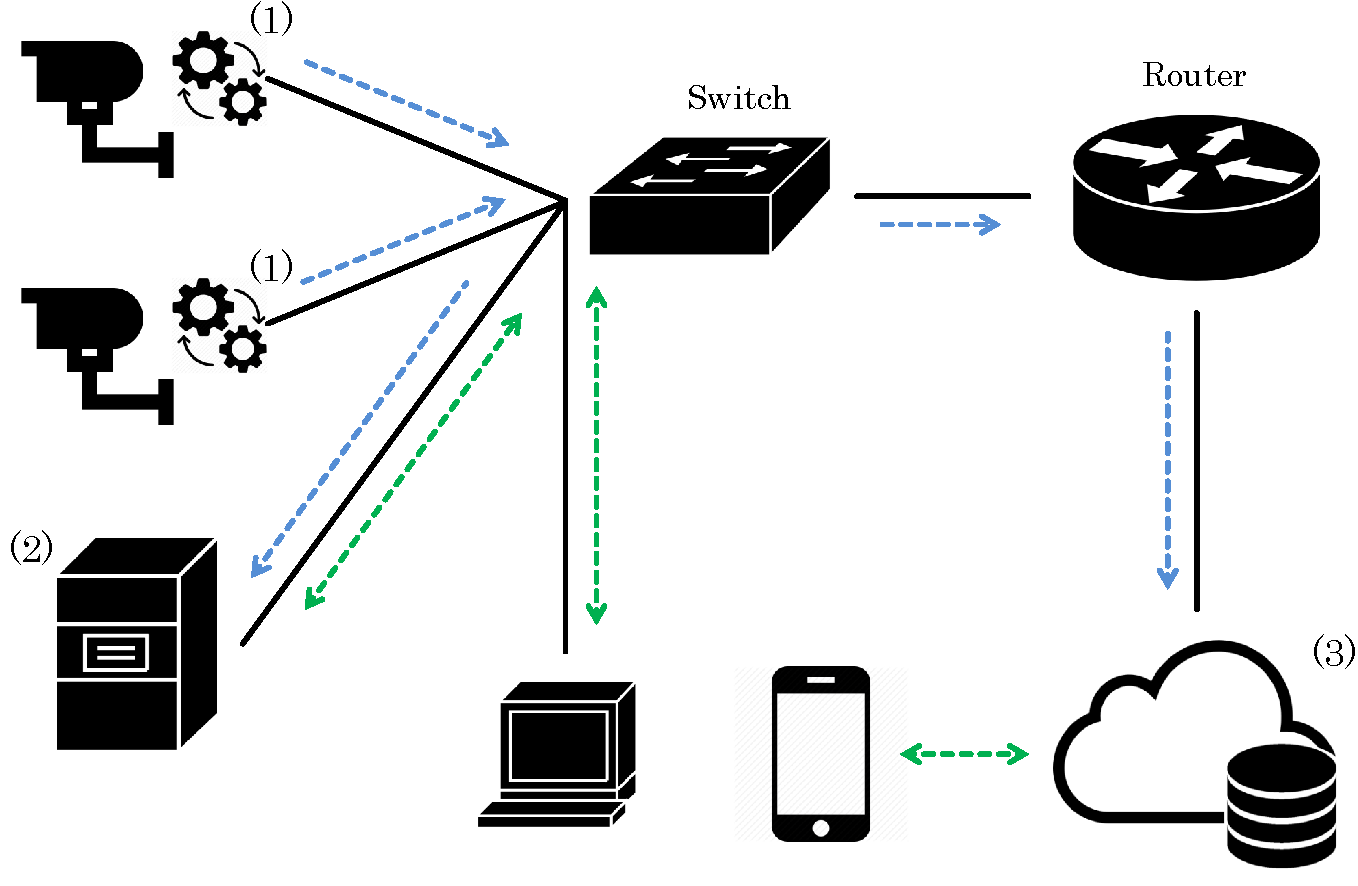
\includegraphics[width=0.8\textwidth]{graphics/cctv/cctvSystem/cctvSystem.pdf}
  \caption[Exemplary structure of a CCTV system.]{Exemplary structure of a CCTV system with two IP cameras. These devices preprocess (1) their captured data before streaming it (blue) to either a local (2) or cloud-based storage (3). Access to the stored video data (green) either stays in the local network or is done through the internet.}
  \label{fig:cctv_system}
\end{figure}

However, while the technology of cameras and the systems surrounding them changed over the years, the challenges still persist: Even while the above mentioned providers provide event detection, these events are merely filtered based on motion detection, therefore many events are constantly being detected, most of them being normal and not of interest. Traditional ways of anomaly detection in video requires either requires human monitoring of the video feeds 24/7, which is inefficient, or going over the stored video data in intervals to look out for anomalies. The latter one is not desired due to the delay until an event of interest is detected; this might even cost lives in some use case scenarios \cite{ferenbok2013hidden}. Also, because it is easier to setup cameras for CCTV systems, the number of video feeds that need to be analyzed in even small CCTV systems has also increased over the years \cite{vlahos2009surveillance}.  This increasing demand for automatic methods for analyzing the increasing quantities of video data that is continuously being generated, warrants the application of various machine learning techniques to detect anomalies. In the following section, we explain and discuss the types of anomalies and how they appear in video streams and how different anomaly detection techniques would work for the given problem and how they differ from each other.



% Anomaly Detection
\section{Anomaly Detection} \label{sec:anomaly_detection}

Anomaly or outlier detection, describes the recognition of patterns that do not comply with the general expected behavior, as illustrated in Figure \ref{fig:anomalies}. The research areas of thereof include machine learning, statistics, information theory, among many others and the application domains are also wide ranging and it is often non-trivial \cite{chandola2009anomaly}: Detected anomalies are not necessarily malicious activities in the context of a security application for example, but it could be the case, that these anomalous observations are merely an unknown and new, but a to be considered normal kind of pattern within the data. In addition, true anomalies might be detected as normal observations, if they are similar to past normal ones. This challenge increases, when normal and anomalous behavior evolves over time and the detection technique has to evolve with it. Although the application domains differ from each other, the challenges remain the same and this includes video anomaly detection (VAD) \cite{shin20203d}.

\begin{figure}
	\centering
	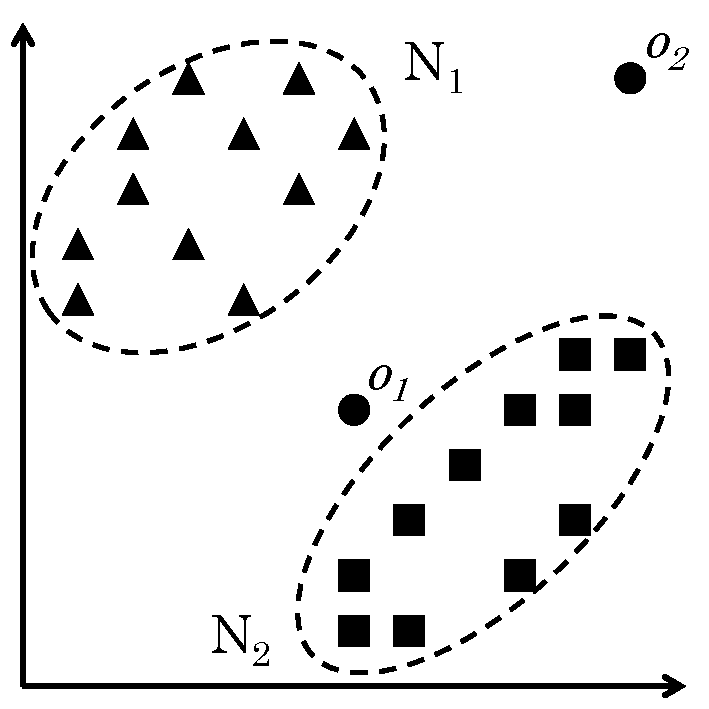
\includegraphics[width=0.39\textwidth]{graphics/anomalyDetection/anomalies/pointAnomaly/pointAnomaly.pdf}
  \caption[Example of outliers in a 2-dimensional data set.]{Example of outliers ($o_1$, $o_2$) in a 2-dimensional data set. \cite{chandola2009anomaly}}
  \label{fig:anomalies}
\end{figure}

In this section, we provide the categorization for the types of anomalies and how they relate to anomalies found in video streams. Due to their nature, a different definition of the types of anomalies based on object patterns is also added to that. For the detection of anomalies within video streams, different detection techniques could be used, determined by the existence and the properties of training data and how the video streams have to be analyzed. Therefore, a taxonomy of the different types of anomaly detection techniques is given, and the challenges that come with them for VAD are highlighted.


% Types of Anomalies
\subsection{Types of Anomalies} \label{subsec:anomaly_types}

An important aspect of anomaly detection is the nature of the (to be) detected anomalies. These can be divided into the following three categories \cite{chandola2009anomaly}:

\paragraph{Point Anomalies} \label{par:point_ano}
The simplest type of anomaly and often the main focus of many research on anomaly detection \cite{malik2014comparative}: These anomalies are considered anomalous on its own with respect to the rest of the data. See Figure \ref{fig:anomalies} for exemplary anomalies $o_1$ and $o_2$. In an example from an application domain, a point anomaly could be a credit card transaction, in which the amount spent is much higher compared to normal transactions. Point anomalies are often not of interest in VAD \cite{shin20203d}. This is because videos are considered spatio-temporal in nature, i.e. they do have a temporal component and the observations --- video frames, are heavily dependent on past and future frames, which results in many anomalies being either contextual or collective. However, they do exist and they can be artificially injected; for our evaluation data set that is presented in detail in Chapter \ref{chap:contribution}, we created a few of these anomalies, by adding flashing of lights during the recording.

\begin{figure}
	\centering
	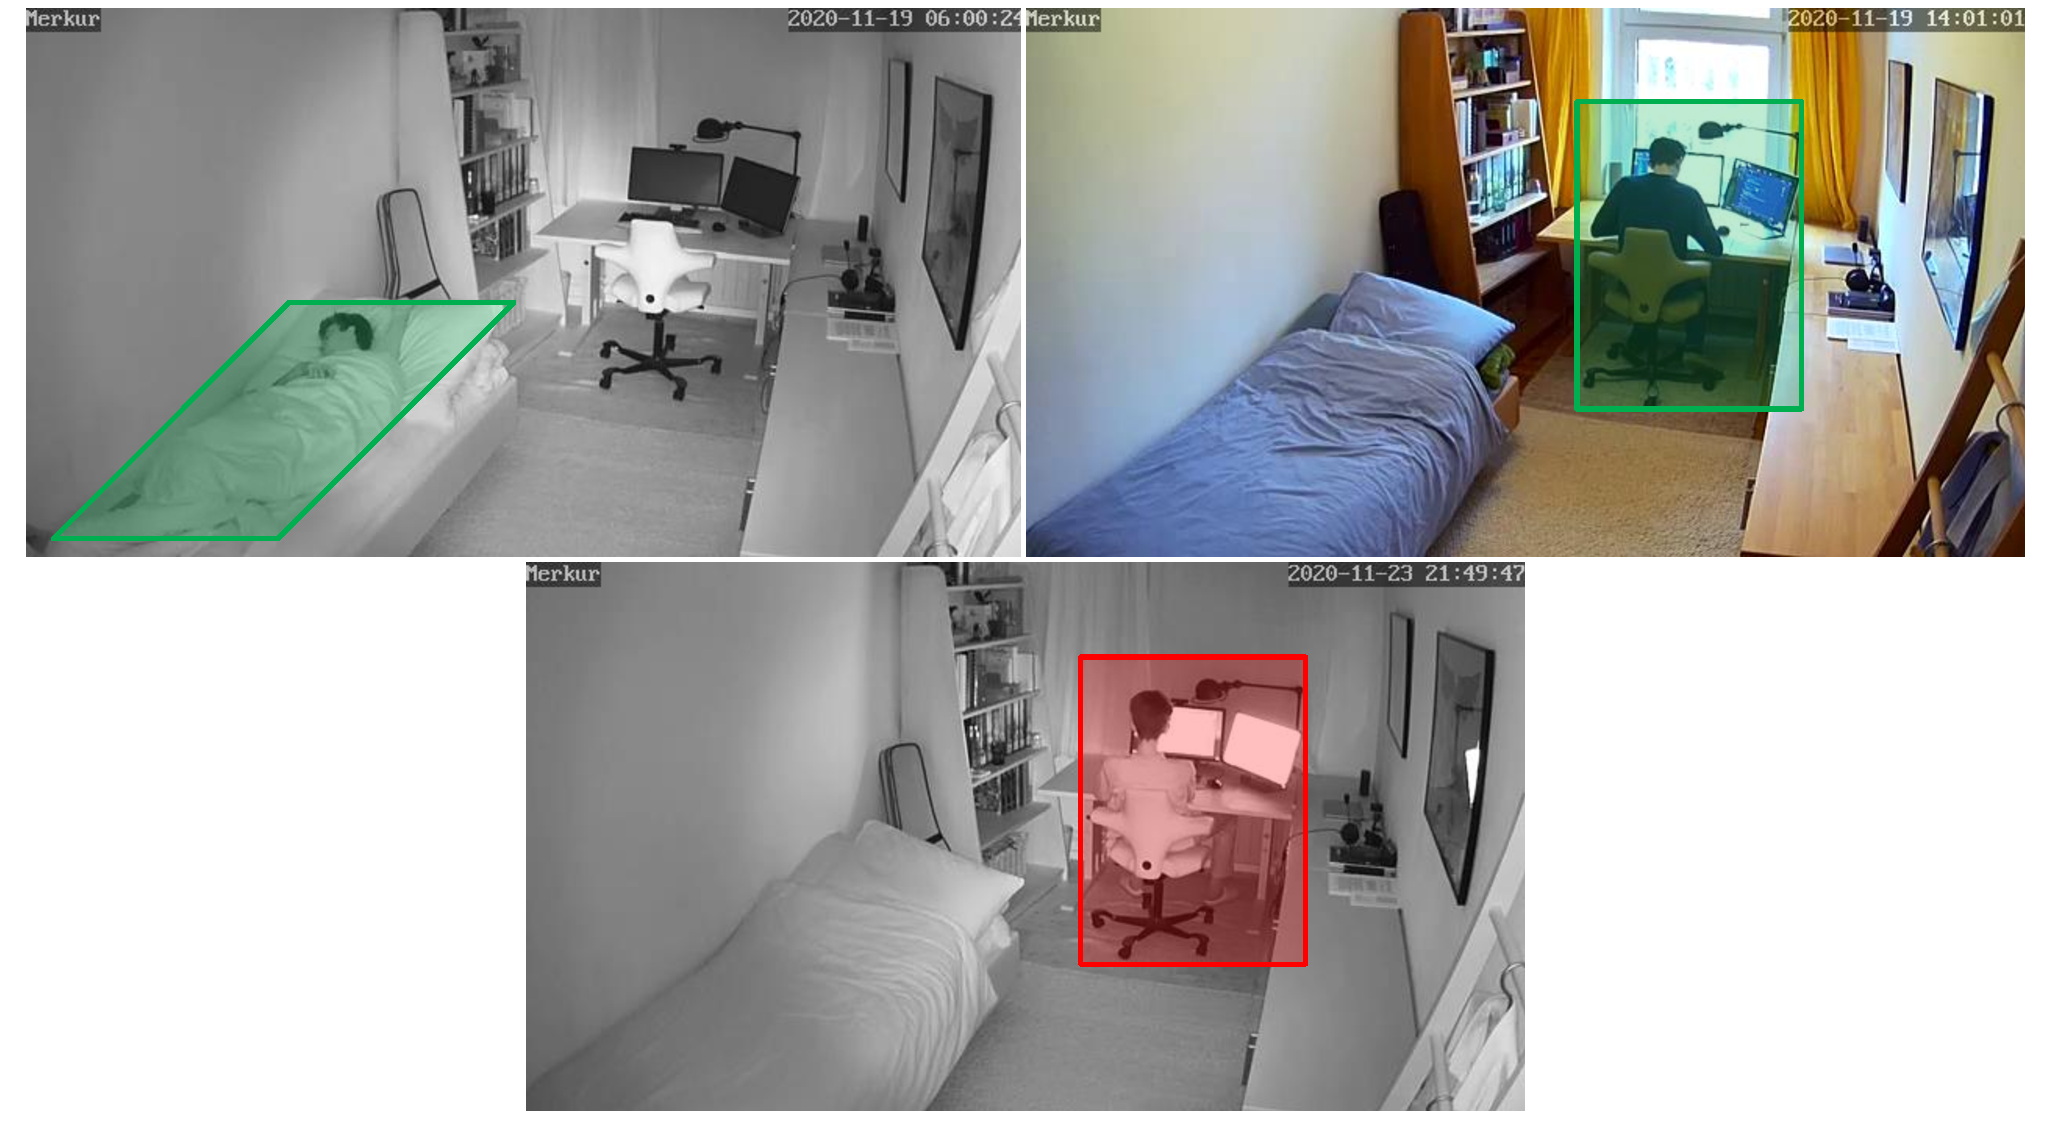
\includegraphics[width=0.68\textwidth]{graphics/anomalyDetection/anomalies/contextualAnomaly/contextualAnomaly.pdf}
  \caption[Contextual anomaly in video.]{A normal video frame during the night (upper left), the day (upper right), and a contextually anomalous one (lower middle). The object pattern marked in red is anomalous at night but normal under other circumstances.}
  \label{fig:contextual_vid_anomaly}
\end{figure}

\paragraph{Contextual Anomalies} \label{par:context_ano}
The notion of a context is usually induced by the data and the use case itself; they are most commonly found in time-series data which is spatio-temporal, same as video streams. These observations are considered normal during one context, while being anomalous in another. In case of a time series, the context can be directly encoded into the observation as a contextual attribute, which enables a detection system to detect these like point anomalies. In video however, defining a context is not always trivial, because there can be several different contextual attributes. First, patterns of objects in a video are often the case for contextual anomalies \cite{shin20203d}: A person walking on the cross-walk or sidewalk is considered normal, but when the same pedestrian is walking on the street it is an anomaly. Because both its appearance and motion pattern differ to the cars surrounding it. Second, as shown in Figure \ref{fig:contextual_vid_anomaly}, the behavior of the person can also depend on the light levels, or the time of day. In that case, when the curtains are closed and the room is not lit, a person sitting at the desk would be a contextual anomaly. Because the context is not explicitly given to the anomaly detection system, the model needs to learn to decode and identify the contexts of the video itself.

\begin{figure}
	\centering
	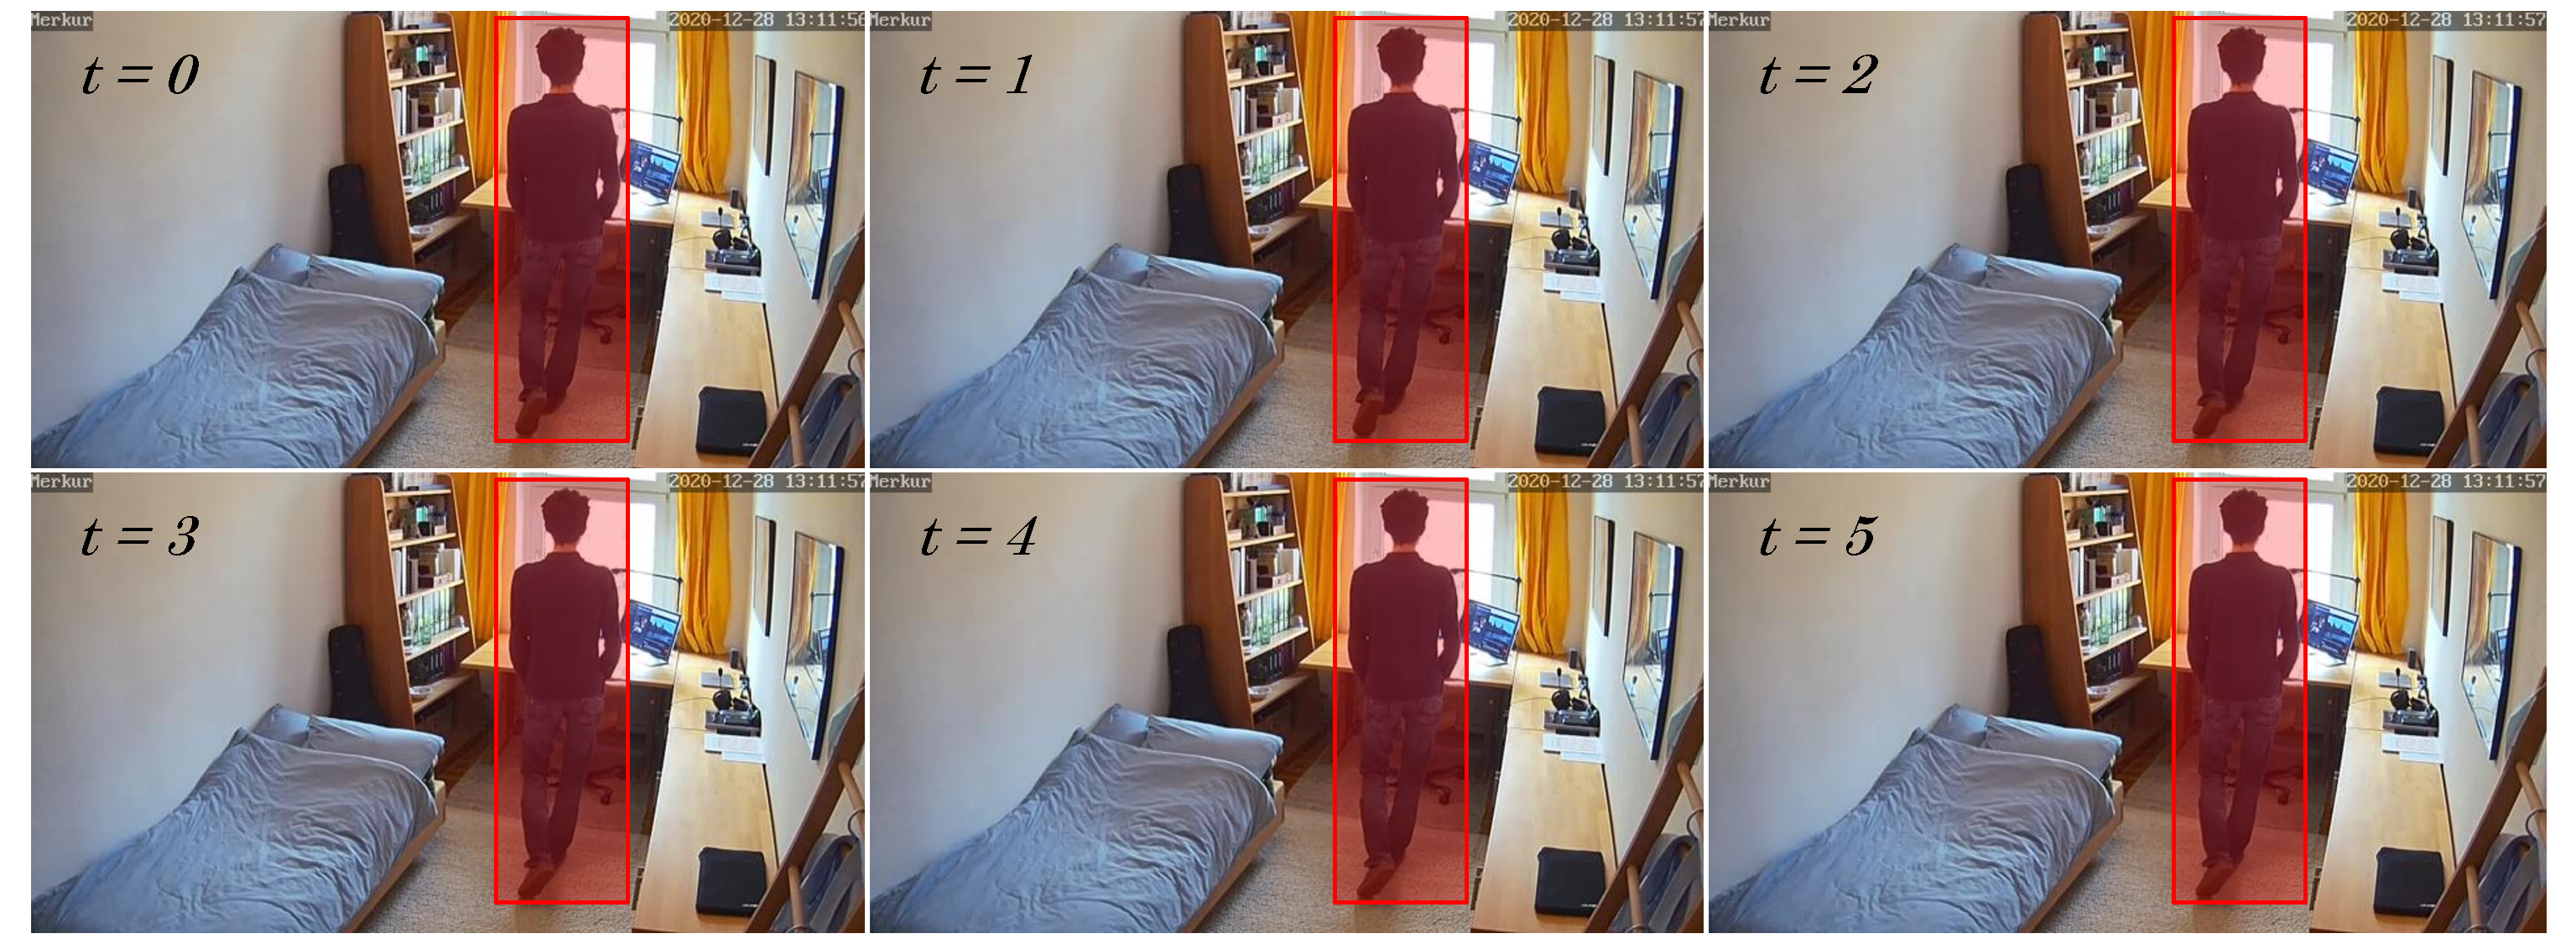
\includegraphics[width=1\textwidth]{graphics/anomalyDetection/anomalies/collectiveAnomaly/collectiveAnomaly.pdf}
  \caption[Collective anomaly in video.]{Individually these consecutive frames would be classified as normal, but together they are considered collectively anomalous. Although the person (red) seems to be walking, they are actually standing still.}
  \label{fig:collective_vid_anomaly}
\end{figure}

\paragraph{Collective Anomalies} \label{par:collect_ano}
Sequence data, such as video streams, sometimes has observations that look normal on their own, but with respective to observations that came before and will come after them, they are anomalous. An example from an intrusion detection system is the patterns of certain attacks, which consist of normal looking events \cite{chandola2009anomaly}. In video, collective anomalies can be detected by the motion patterns of the objects in a video: While the individual frames shown in Figure \ref{fig:collective_vid_anomaly} appear normal --- the person is walking from the camera away and towards the desk. Or so it seems. Because when one inspects the preceding and succeeding frames, one notices that the person is standing still. Vice versa, a very fast motion of an object that under normal circumstances moves more slowly could be considered a collective anomaly instead --- the collection of frames of that motion being part of that anomaly. Thus, a VAD system needs to learn to extract spatio-temporal features of objects within the video, i.e. it needs to learn how objects move under normal circumstances. Finally it is to note, that collective anomalies can also be contextual; a group of observations might be considered collectively anomalous in a specific context (e.g. a person running over the sidewalk), while in another context that motion pattern would be considered normal (e.g. the same person running over the sidewalk while it rains).


% Differentiating between Techniques
\subsection{Taxonomy of Anomaly Detection Techniques} \label{subsec:detection_techniques}

\paragraph{Detection Output} \label{par:detect_out}
The main requirement of an anomaly detection system is to report observations that appear anomalous. This either means that the system labels each observation in binary fashion, or that the underlying results are aggregated and smoothed over, to group the individual reports into events that are either normal or anomalous \cite{chandola2009anomaly, malik2014comparative}. Some detetion systems go further, and replace the binary output with a mapping to the specific kind of anomaly that was detected. Often however the results from the detection system is neither of the two but it is a score, ranging from $0$ and $1$, depending on the probability to which the model considers that instance an anomaly. In that case, the results are either mapped to a binary label by an expert, or a domain specific threshold function is defined by them. Our ADS for video presented in the next chapter does use a scoring technique internally, but due to the use of IFTM, a threshold is applied to the result which results in a binary label output \cite{schmidt2018iftm}.

\paragraph{Level of Supervision} \label{par:supervision}
Second, depending on the nature of training data and its labels --- in case of anomaly detection binary ones (normal or anomalous), it is decided which anomaly detection techniques can be used. This is because most outlier detection solutions need to be trained one some observations, before they can be used to detect outliers \cite{Bishop2006patttern, chandola2009anomaly}. And, depending on the detection approach, these have different requirements to the training data instances. The most transparent approaches to humans are policy-based, also called rule-based techniques \cite{huebscher2008survey}. By constantly checking if policies and rules, that were written by system administrators for example, are upheld, anomalies are detected if one or multiple of these rules are broken by the parameters of the system that is observed. Defining these rules can be simple for smaller systems and some application domains, but for others it becomes increasingly difficult if not impossible. But as already noted in the previous paragraph regarding the detection output, the output of a technique can be refined by the rules and policies of the human operator. For example in the case of the CCTV system by Netatmo that was presented in Section \ref{sec:cctv}, events are generated if successive frames differ from each other by a human set threshold $T$. Then, a facial recognition model is run on any detected humans and if these faces do not match with an internal database for that household that is monitored, the system interprets this behavior a breaking in policy and an alert is generated. However these underlying models are still trained in some fashion and therefore these techniques are not purely policy driven.

Then, there are supervised learning techniques; these require to be trained by labeled data of all existing normal and anomalous behavior. A prime example of this method is the nearest neighbor algorithm, that assigns every new incoming observation to the label of the nearest sample in the training data set \cite{cover1967nearest}. This techniques can provide the best results when there is a sufficient number of training data, but obtaining accurate and representative labels can be challenging, especially for surveillance data. For the rarest types of anomalies, this would imply some catastrophic events, that are very difficult to collect \cite{chandola2009anomaly}. In addition, labeling any kind of data is very expensive, due to the need of some human expert to label the observations by hand. For our use case as described in the following chapter, several days of unlabeled video data was available to us, but none of which was actually labeled.

This challenge of lacking labeled data transfers to the next kind of learning technique; semi supervised learning. In this case, models are either trained with a combination of labeled and unlabeled data, or only with the observations that show one type of class. In the latter case, a model based on the normal behavior of a system can be built \cite{malik2014comparative}. On the other hand, some models use forms of transfer learning to infer the labels of the remaining (unlabeled) training data, to refine the model further, after which it has been trained by the labeled observations \cite{shin2018cctv, shin20203d}. In Chapter \ref{chap:state_of_the_art}, we will discuss some research regarding these approaches and discuss how they differ from our own solution.

For unsupervised anomaly detection, no labels at all are available during training. These makes them widely applicable, because for training, raw data can be fed to them. However this does come with a price, because they often run under the implicit assumption, that anomalies are rare and thus are ``drowned out`` during training, because the normal data dominates the set. If this assumption is done falsely, the detection rate of these techniques will suffer \cite{chandola2009anomaly}. For VAD systems, this assumption is often made \cite{schlegl2017unsupervised, jamadandi2018predgan, akcay2018ganomaly, liu2018future} due to the high availability of raw data. Our proposed video generation model is trained in unsupervised fashion, as is IFTM in which the model is incorporated after training \cite{schmidt2018iftm}. 


\paragraph{Online or Offline} \label{par:online_offline}
Finally, anomaly detection algorithms can be divided into two groups, into which all algorithms that require input fall \cite{karp1992line}: Pure offline detection techniques require the entire batch --- data, that has to be analyzed beforehand. This can yield better results due to their encompassing view of all observations, but at a cost of being no longer able to detect anomalies in real-time, but only after these have occurred. Others group incoming observations into smaller sets called mini-batches and process these indivudally in a batch wise manner to solve this problem, but in return they lose some detection quality. The most responsive systems are online algorithms. These are especially useful for continuous streams of observations that have to be analyzed one step at a time. Video feeds generated by a camera are one of these use cases, because the size of the potential data set is technically infinite. Though, online techniques are more responsive compared to offline methods, they struggle especially at the start --- this is called the cold start problem, when their models are not that good due to the lack of sufficient training initially. Furthermore, context shifts within the data stream can occur, forcing the model that no longer represents the incoming data, to adapt to the new context. This requires the model to recognize the shift and then to either use a new model, or to forget older observations that are no longer relevant to the current state. These two groups should not be seen as binary --- training could be realized as a batch process over a set of observations that is known in advance, before the incoming stream of observations is classified in real-time. In some cases, the underlying model is also trained on a batch of data in advance, before it is further refined in stream-wise fashion, while also already classifying the new incoming observations. This kind of pre-training counteracts the cold start problem \cite{erhan2010does}.

The anomaly detection framework that is used in our approach --- IFTM, is flexible \cite{schmidt2018iftm}: Its threshold model can either be trained offline and is then fixed for the detection phase, or it can be continuously updated online-wise. But, because our model that represents the normal state of the video stream is trained in adversarial fashion until convergence \cite{goodfellow2014generative}, as explained in the following section, training of the entire system has to be done offline. Therefore the entire video ADS is doing training offline and detection will be done in an online manner.



% GANs
\section{Generative Adversarial Networks} \label{sec:gans}

Over the last years, research moved away from typical neural networks \cite{haykin1994neural} to more refined deep neural networks that are able to recognize high level concepts, such as objects in images or videos, audio waveforms containing speech, or the processing and understanding of written text \cite{bengio2009learning}. This change was also made possible due to the increasing power of modern hardware and distributed computing, which allowed an increase in complexity of the networks. The abstract underlying concepts remain the same however; the variables within a network are optimized following certain criteria that rate the quality of the outputs that the model produces. Backpropagation is then used to calculate the gradients, and these are then passed to an optimization algorithm to adjust the trainable parameters within the network.

With the increasing complexity and thus the increase in trainable parameters, there is the increasing risk that components of the inputs during training are directly copied into the network's parameters. Goodfellow et al. claim generative adversarial networks (GANs) overcome some of these challenges \cite{goodfellow2014generative}. GAN --- as the name suggests, consists of atleast two neural networks, that are adversaries in nature. As one can see in Figure \ref{fig:gan}, the generative model (the generator) is pitted against a counterpart (the discriminator). The latter one has to learn the properties of the training data and to distinguish real inputs that have these properties from synthetic ones. The generator on the other hand has to learn to trick its opponent into believing that its synthetic outputs are real enough to be labeled as not fake. 

\begin{figure}
	\centering
	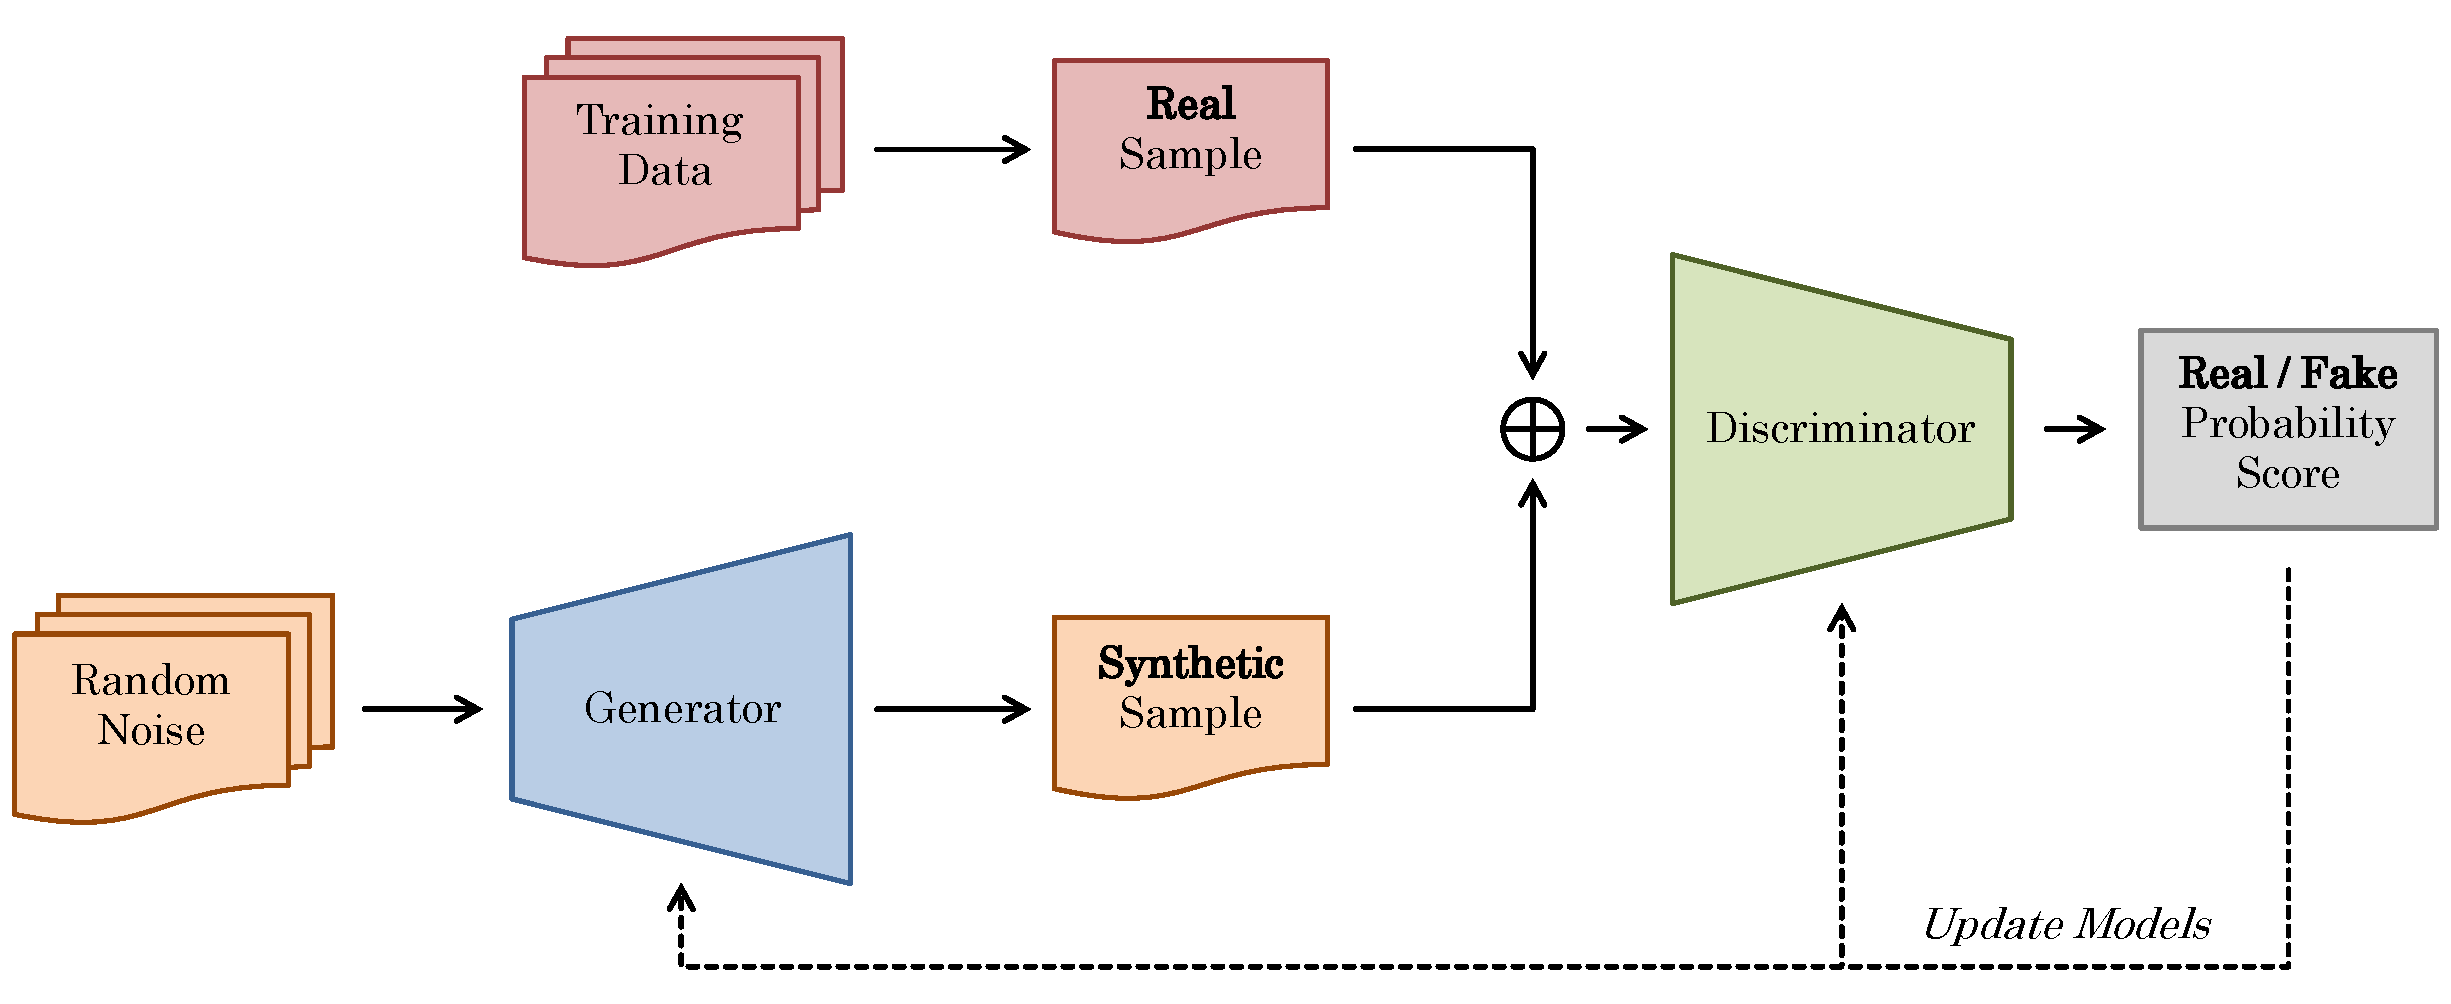
\includegraphics[width=1\textwidth]{graphics/gan/gan/gan.pdf}
  \caption[Structure of a GAN.]{Exemplary structure of a GAN. Synthetic samples are generated based on inputs sampled from random noise. Classification results for synthetic and training samples by the discriminator are used to tune the two models.}
  \label{fig:gan}
\end{figure}

This approach during training can be formalized into Equation \ref{eq:gan}, with the generator network being $G$ and $D$ being the discriminator: The first term describes the error of $D$ to recognize inputs $x$ sampled from the training distribution $p_x$, and labeling these as real ($D(x)=1$). Therefore the discriminator gains direct insight into the training data set. This is usually done in an unsupervised manner; the learning of any features and properties that make these observations real is the overarching goal during training. There are also variations of GAN in which the discriminator learns to not label inputs as either real or fakes ones, but to provide non-binary classification \cite{simonyan2014two, isola2016image}. The second term in the Equation refers to the sampling of $z$ from a normal distribution, that is passed to the generator to generate a synthetic output. This output is then classified by the discriminator. The goal of the generator is to minimize this term, i.e. $D$ must no longer be able to discriminate between real and synthetic data points. Meanwhile $D$ seeks to maximize it, labeling synthetic examples as fake ($D(G(z))=0$). Training of GANs is done iteratively; every step, a mini-batch is sampled from both the random distribution ($p_z$) and the training data ($p_x$) and both models are updated separately to optimize Equation \ref{eq:gan}.

\begin{equation} \label{eq:gan}
\min_G \max_D V(D,G) = \mathbb{E}_{x \sim p_x(x)}[\log D(x)] + \mathbb{E}_{z \sim p_z(z)}[\log(1 - D(G(z)))]
\end{equation}

Thus training GANs is a zero-sum game, in which both models have to improve in parallel. As $D$ becomes better in distinguishing real from fake examples, $G$ also improves in fooling its adversary, making the generated outputs more and more real. This way, the generator, without having direct access to the training data, learns general feature representations that mirrors the statistics of the training set. For example, if one trains a GAN with a database of human faces, the training examples are passed to the discriminator, and the generator will learn to generate real looking human faces from random input $z$. 

\paragraph{Common Failure Modes in GAN Training} \label{par:failure_modes}
Note that the convergence of Equation \ref{eq:gan} should not be one-sided \cite{zhang2018convergence}: If the two sides do not reach a balance during training, one of the two models will slowly minimize their error until the error of that model reaches zero, while the other reaches the error function's maximum. This not only stops improvement in training, but actively degrades the output: In case $D$ dominates during training, $G$ no longer is able to generate any outputs that might fool its counterpart and thus gets no hints on how to continue learning. Vice versa, if $G$ overpowers $D$, the generator usually learns some simple feature representation that the discriminator can not identify as fake. This can also result in generated outputs, that have a low error from the discriminator's point of view, but are very low in quality. Lastly, there is also the ``mode collapse``, in which $G$ no longer generates a large variety of different outputs, but ``collapses`` different input ($z$) to the same synthetic output. This happens if the generator is unable to learn a rich feature representation from the given inputs.

There are different approaches to solve the different failure modes \cite{roth2017stabilizing, zhang2018convergence}. They include the impairment of one model and the improvement of the other. This can be done by simply increasing or decreasing the number of trainable parameters of a model, i.e. adding and removing layers, lowering the dimensions of certain layers, etc.. But an impairment can also be realized by adding regularization layers, such as dropout layers \cite{hinton2012improving}: A dropout layer randomly sets a percentage of the input units of the next layer to 0, which forces the model to add redundancies in its parameters, thereby lowering its expressiveness. When weakening the discriminator, one can also randomly flip the labels of the data from which the discriminator trains from. This can either be done in one-sided manner, labeling real data points as synthetic, or for both classes equally. For solving the mode collapse problem, one can also increase the size of the latent input space. Finally, one can also tune the number of training steps, that each model does per training iteration. So for example, in case $D$ overpowers the training, $G$ is trained two mini-batches during each step, while $D$ is merely trained once.

Although Goodfellow et al. have formally proven \cite{goodfellow2014generative}, that training will always converge, if both models have enough capacity and they are both trained each step until having reached an optimum, this is not necessarily an equilibrium in which both discriminator and generator continuously improve. If the generator succeeds perfectly, while also generating perfect synthetic data points, the discriminator has a 50\% accuracy; the prediction is essentially a coin toss. This feedback however can create an oscillating error, that may start the generator to train on false feedback, thus worsening the generator once more and risking a collapse in training. This can be solved by early stopping, i.e. stopping training once a stable equilibrium was achieved \cite{yao2007early}, but there are also other variants that change the way training is done in dynamic fashion to adapt to the changes in objectives \cite{zhang2018convergence, thanh2020catastrophic}.\\

Our proposed ADS system uses a GAN, namely the generator after training is completed, to model the properties that normal video observations have. Therefore, we design $G$ and $D$ to generate and discriminate videos, respectively. The challenges in training GAN were in some part also encountered during the evaluation of our approach; these challenges are discussed in Chapter \ref{chap:contribution} and \ref{chap:results}. Note that the idea to use GANs for video generation, forecasting, and VAD are not novel; in Chapter \ref{chap:state_of_the_art} we provide an overview over similar approaches to ours. 

The rest of this section provides a short introduction into a constrained architectural variant of GAN, that is more stable for some application domains --- especially image and video generation. Lastly, we provide an overview over a subtype of GANs that accept additional inputs, which is necessary for video generation forecasting.


\subsection{Deep Convolutional Generative Adversarial Networks} \label{subsec:dcgan}

There are different challenges when designing GANs --- some of them are highlighted in Paragraph \ref{par:failure_modes}, which makes the designing of these adversarial models particularly challenging. Due to that, new models are usually based on already existing constrained architectures, that were proven and evaluated to work on different application domains. Deep convolutional generative adversarial networks (DCGANs)\nomenclature{DCGAN}{Deep convolutional generative adversarial network} \cite{radford2015unsupervised} build on the success of regular convolutional neural networks (CNNs)\nomenclature{CNN}{Convolutional neural network}. CNNs have a wide array of applications when processing some form of spatial data \cite{ciregan2012multi}. For example when processing images, pixels that are neighbors are relevant to each other when extracting features out of that image. By sliding kernel filters over an image and aggregating the neighboring pixels values, one can create a number of feature maps from a single input. These feature maps can be aggegrated or further processed by additional convolutional layers to extract lower level features, to be used for image classification or object recognition \cite{krizhevsky2017imagenet}. One can also replace these 2-dimensional convolutions with 3-dimensional ones \cite{tran2015learning, ji20123d}, which allow a model to understand spatio-temporal features. One of the application domains for these is video processing \cite{simonyan2014two}.

\begin{figure}
	\centering	
	\begin{subfigure}{\textwidth}
    \centering
    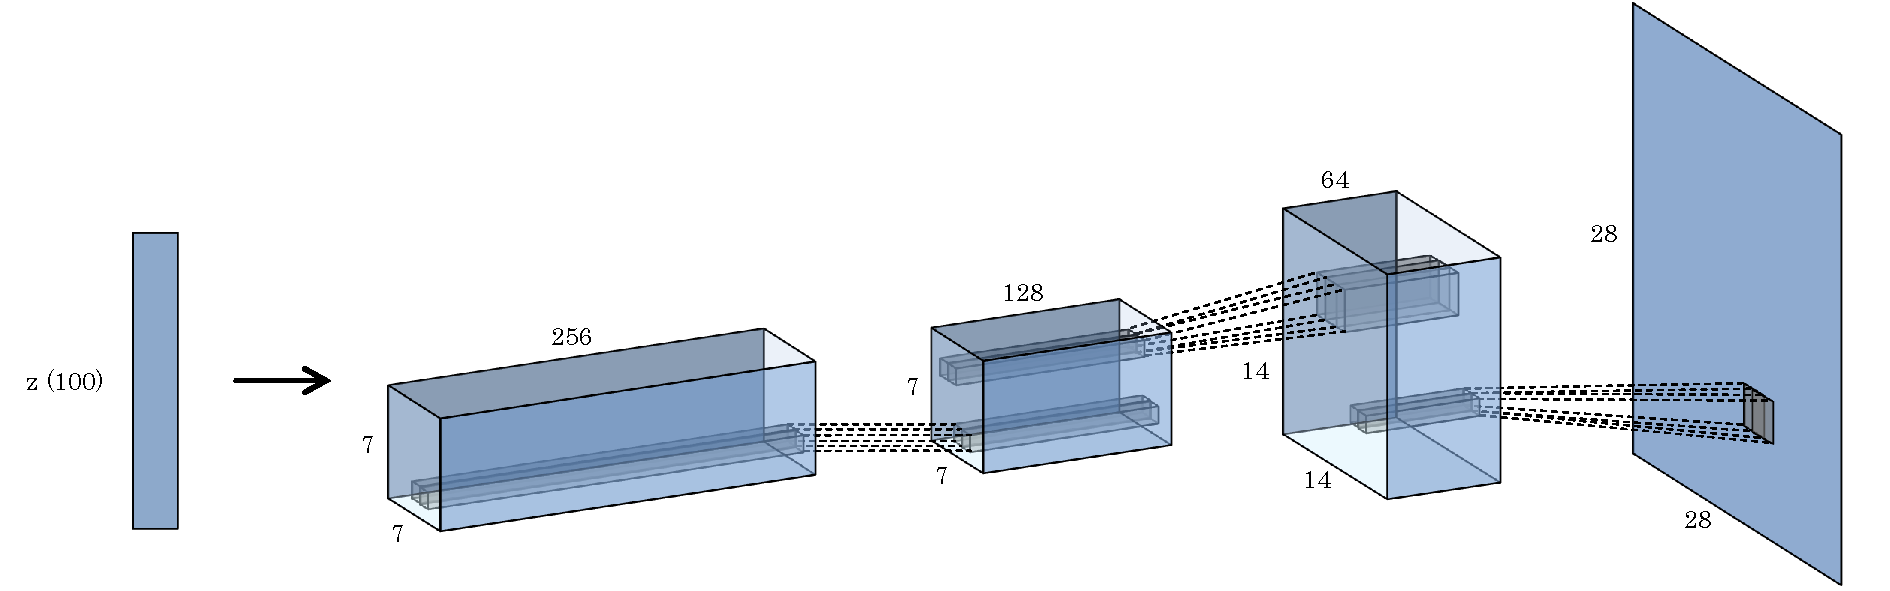
\includegraphics[width=1\textwidth]{graphics/gan/dcgan/dcgan_g.pdf}
    \caption{DCGAN generator.}
    \label{subfig:dcgan_g}
  \end{subfigure}
 
	\begin{subfigure}{\textwidth}
    \centering
    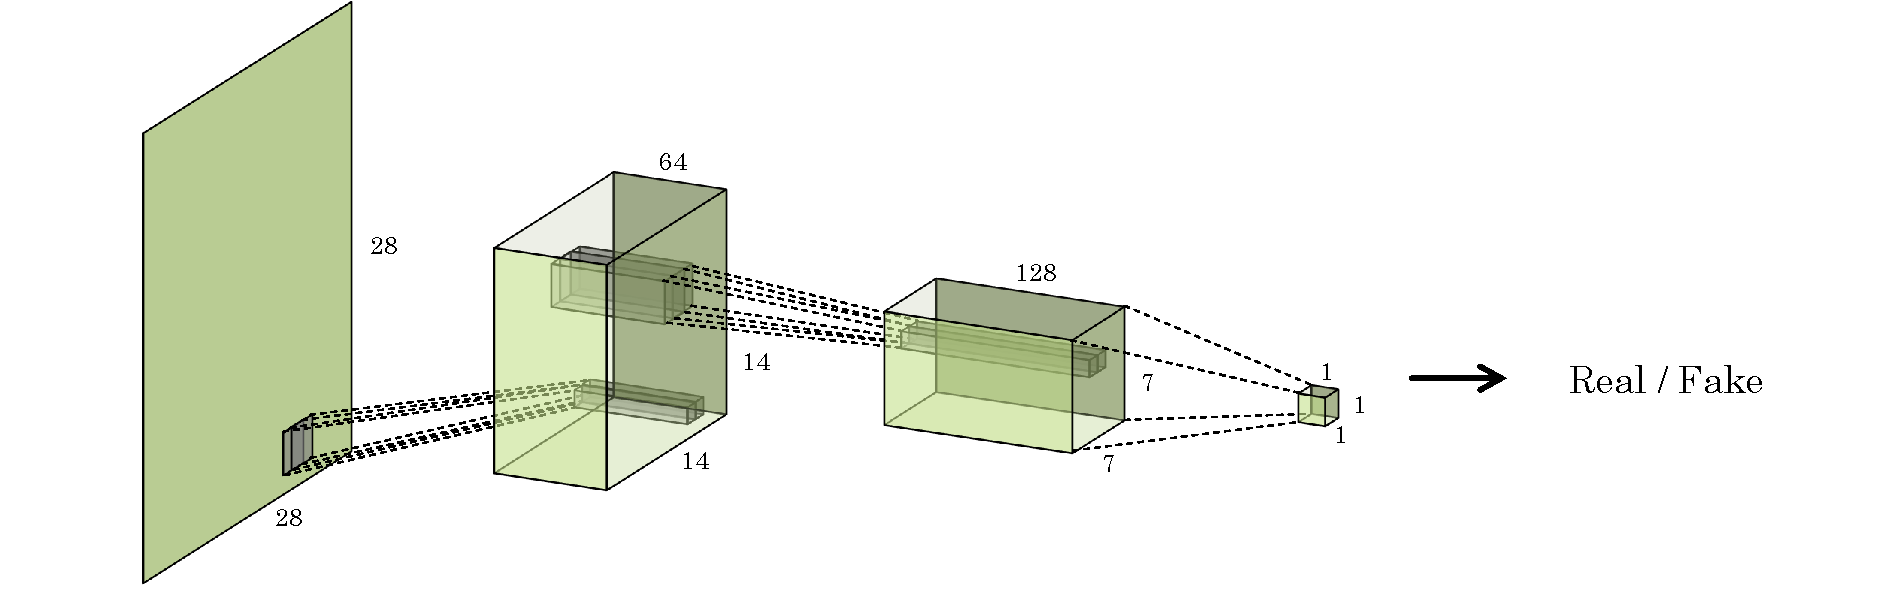
\includegraphics[width=1\textwidth]{graphics/gan/dcgan/dcgan_d.pdf}
    \caption{DCGAN discriminator.}
    \label{subfig:dcgan_d}
  \end{subfigure}
  
  \caption[Constrained DCGAN architecture.]{Exemplary DCGAN for image generation and discrimination. A 100-dimensional random latent vector is projected and reshaped to a small convolutional representation but with many feature maps (pictured by the depth of each cuboid). Three fractionally-strided spatial convolutions then upsample the encoded representation into a $28 \times 28$ grayscale image. The discriminator reverses this process, downsampling the image to a 1-dimensional output.}
  \label{fig:dcgan}
\end{figure}

Radford et al. combine CNNs with their counterpart --- de-convolutions often called, that instead of increasing the number of filters while usually decreasing the size of the dimensions, do the opposite. This technique can be used for upscaling \cite{zeiler2010deconvolutional}. The discriminator ($D$) in this architecture is therefore a CNN-based classifier, and the generator ($G$) creates synthetic output by upsampling the latent input to the output size. This results in two symmetric models as illustrated in Figure \ref{fig:dcgan}\footnote{The DCGAN in the figure is modeled after the one used in the DCGAN TensorFlow tutorial (\url{www.tensorflow.org/tutorials/generative/dcgan}), which generates ``hand-drawn`` MNIST digits \cite{lecun2010mnist}.}. DCGAN however has more constraints for its architecture: First, pooling layers, that are usually applied after a convolutional layer to aggregate the outputs, are replaced by strided (for $D$) and fractionally-strided (for $G$) convolutions. Changing these deterministic layers to something that can be trained, allows the models to learn their own downsampling and upsampling, respectively \cite{springenberg2014striving}. Any fully connected hidden layers are also removed, except for the input of the generator and the output of the discriminator. Batch normalization layers \cite{ioffe2015batch} are used after every layer in both $D$ and $G$ except for the input and the output, respectively. According to Radford et al., this prevents early mode collapse \cite{radford2015unsupervised}. Using only bounded activation functions, such as ReLU \cite{nair2010rectified} for the generator and Leaky ReLU \cite{maas2013rectifier} for the discriminator instead of maxout activation like in original GAN, except for the generator output layer that uses the hyperbolic tangent activation, also creates better results when using GANs for spatial data \cite{radford2015unsupervised}. Finally during training, no pre-processing steps for the input data was taken, besides scaling it to a range of $[-1,1]$. For the optimization of the trainable parameters the Adam optimizer \cite{kingma2014adam} with tuned hyperparameters was chosen.

Although the reference architecture on which our approach built is based on DCGAN, we evaluate different hyperparameter combinations for the batch size and the optimizer's learning rate for the adversarial training of our model. Both our model, use case, and data differ, while the parameters for DCGAN in the original paper were chosen for specific data sets, mainly image and face generation. The underlying idea of the DCGAN architecture is preserved though. The differences of the chosen parameters to those described here are further expanded on in the next chapter.


\subsection{Conditional Generative Adversarial Networks} \label{subsec:cgan}

Lastly it is to note, GANs are not only useful for generating real looking synthetic images and other outputs, but by tuning the function which has to be optimized, one can set different goals for the models that are trained. Mirza and Osindero adapt Equation \ref{eq:gan} to condition both models on predetermined, non-random input, resulting in Equation \ref{eq:cgan} \cite{mirza2014conditional}. $y$ in that case can be seen as additional information which $G$ and $D$ use to generate or discriminate data. In case of the generator this means, that the sampled noise $z$ is combined with $y$. Because the discriminator gets $y$ as an input as well, $G$ will implicitly learn to generate outputs, that somehow relate to $y$. In case of MNIST digits \cite{lecun2010mnist}, this could mean telling the generator to generate a specific type of digit ($y$). But this can also be extended by giving the conditional generative adversarial network (C-GAN)\nomenclature{C-GAN}{Conditional generative adversarial network} a list of tags that should be used as a baseline to generate an image from.

\begin{equation} \label{eq:cgan}
\min_G \max_D V(D,G) = \mathbb{E}_{x \sim p_x(x)}[\log D(x|y)] + \mathbb{E}_{z \sim p_z(z)}[\log(1 - D(G(z|y)))]
\end{equation}

For out approach, we use a variant of this method to give the generator conditional input in the form of spatio-temporal data (video frames), and it will learn to generate future frames from it. This is explained in detail in the following chapter, Section \ref{sec:cvgan}.